\documentclass{standalone}


\usepackage{tikz}
\usetikzlibrary{arrows,arrows.meta,shapes}

\begin{document}
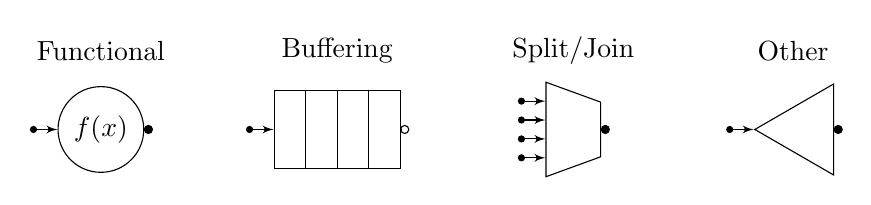
\begin{tikzpicture}[auto, node distance=1cm,>=latex']

\tikzset{
    triangle/.style={
        draw,
        shape border rotate=180,
        isosceles triangle,
        isosceles triangle apex angle=60,
				minimum height=1cm
    }
}


\node[circle,draw,minimum size=1cm] (fun) {$f(x)$};
\node[above of = fun] {Functional};
\draw [{Circle[scale=.7]}->] ([xshift=-.35cm]fun.west) -- (fun.west);
\draw [-{Circle[scale=.9]}] (fun.east) -- ([xshift=.11cm]fun.east);


\node[rectangle,draw,minimum height = 1cm, minimum width=1.6cm,right of = fun, xshift=2cm] (buf) {};
\node[above of = buf] {Buffering};
\draw ([xshift=-.4cm]buf.north) -- ([xshift=-.4cm]buf.south);
\draw (buf.north) -- (buf.south);
\draw ([xshift=.4cm]buf.north) -- ([xshift=.4cm]buf.south);
\draw [{Circle[scale=.7]}->] ([xshift=-.35cm]buf.west) -- (buf.west);
\draw [-{Circle[open,scale=.9]}] (buf.east) -- ([xshift=.11cm]buf.east);

\node [trapezium, trapezium angle=70, minimum width=1.2cm, draw, right of = buf, xshift=2cm,rotate=-90] (sj) {};
\node[above of = sj] {Split/Join};
\draw [{Circle[scale=.7]}->] ([xshift=-.35cm,yshift=.36cm]sj.south) -- ([yshift=.36cm]sj.south);
\draw [{Circle[scale=.7]}->] ([xshift=-.35cm,yshift=.12cm]sj.south) -- ([yshift=.12cm]sj.south);
\draw [{Circle[scale=.7]}->] ([xshift=-.35cm,yshift=-.12cm]sj.south) -- ([yshift=-.12cm]sj.south);
\draw [{Circle[scale=.7]}->] ([xshift=-.35cm,yshift=-.36cm]sj.south) -- ([yshift=-.36cm]sj.south);
\draw [-{Circle[scale=.9]}] (sj.north) -- ([xshift=.11cm]sj.north);

\node[triangle,draw,right of = sj, xshift=2cm] (misc) {};
\node[yshift=1cm,xshift=.5cm,at={(misc.west)}] {Other};
\draw [{Circle[scale=.7]}->] ([xshift=-.35cm]misc.west) -- (misc.west);
\draw [-{Circle[scale=.9]}] (misc.east) -- ([xshift=.11cm]misc.east);
    %
\end{tikzpicture}

\end{document}